

\textbf{Квазимонохроматичность}. 
Если область $\Delta \omega$ в которую входит 
% $p.\, v.$
 основное значение интеграла Фурье, и $\Delta \omega / \omega \ll 1$, то результирующее колебание называется \textit{квазимонохроматическое}. Запишем произвольные квазимонохроматические колебания в виде
\begin{equation*}
    E(t) = a(t) e^{i \omega_0 t},
\end{equation*}
где $a(t)$ -- медленная амплитуда, таким образом колебания модулированы, меняется $a(t)$ -- амплитудная модуляция, меняется фаза -- \textit{фазовая модуляция}. 


Так как детекция происходит в основном для интенсивности, то про неё и будем гворить, квадрат поля может быть представлен в виде
\begin{equation*}
    (\Re E)^2 = \left(\frac{E + E^*}{2}\right)^2 = \frac{1}{4} \left(E^2 + E^{*2}\right) + \frac{1}{2} E E^*.
\end{equation*}
Если считать $a = a_0 (t) e^{i \delta(t)}$, где $a_0(t)$ и $\delta(t)$ -- межденно меняющиеся вещественная амплитуда и фаза, то
\begin{equation*}
    E^2 + E^{*2} = 2 a_0^2 \cos\left[2(\omega_0 r + \delta)\right],
\end{equation*}
что быстроосциллирует, так что $0$. Поэтому интенсивность $\langle E E^*\rangle$. 



\textbf{Два источника}.
Рассмотрим теперь сумму колебаний от двух источников из $S_1$ и $S_2$ с отставваиями на $\theta_1$ и $\theta_2$. Тогда результирующее 
\begin{equation*}
    E \equiv E(P, t) = E_1(t-\theta_1) + E_2 (t-\theta_2).
\end{equation*}
Умножая на комплексно-сопряженное и усредняя по времени приходим к выражению вида
\begin{equation*}
    I = I_1 + I_2 + 2 \sqrt{I_1 I_2} \Re\left[f_{12}(\theta)\right],
\end{equation*}
где $\theta = \theta_2-\theta_1$. 

\begin{to_def}
    \textit{Корреляционной функцией} колебаний $E_1(t-\theta_1)$ и $E_2(t-\theta_2)$ называют 
    \begin{equation*}
        \left\langle 
            E_1(t-\theta_1) E_2^* (t-\theta_2)
        \right\rangle = \left\langle E_1(t) E_2^* (t-\theta)\right\rangle = F_{1, 2}(\theta) = \sqrt{I_1 I_2}f_{1,2} (\theta).
    \end{equation*}
    Она характеризует степень согласованности колебаний. Функция $f_{1, 2}$ называется \textit{нормированной корреляционной функцией}. Разделив её на быстро осциллирующую функцию $e^{i \omega_0 t}$ можем перейти к \textit{комплексной степени когерености колебаний}
    \begin{equation*}
        \gamma_{1,2}(\theta) = f_{1, 2} (\theta) e^{-i \omega_0 \theta},
    \end{equation*}
    модуль которой -- степень когерентнсоти колебаний в точке $P$. 
\end{to_def}



Итого, в терминах $\gamma$, переходим к
\begin{equation*}
    I = I_1 + I_2 + 2 \sqrt{I_1 I_2} \Re\left[\gamma(\theta) e^{i \omega_0 \theta}\right] = 
    I_1 + I_2 + 2 \sqrt{I_1 I_2}  |\gamma_{1,2}(\theta)| \cos(\omega_0 \theta + \delta(\theta)),
\end{equation*}
где $\gamma_{1,2} (\theta) = |\gamma_{1, 2}|e^{i \delta}$. Однако $\gamma$ меняется медленно, так что в максимумах $\cos(\omega_0 \theta + \delta) = +1$ и в минимумах $\cos(\omega_0 \theta + \delta) = -1$, тогда
\begin{equation*}
    \sub{I}{max} = I_1 + I_2 + 2 \sqrt{I_1 I_2} |\gamma_{1, 2} (\theta)|,
    \hspace{5 mm} 
    \sub{I}{min} = I_1 + I_2 - 2 \sqrt{I_1 I_2} |\gamma_{1, 2} (\theta)|,
    \hspace{0.5cm} \Rightarrow \hspace{0.5cm}
    V \equiv \frac{\sub{I}{max}-\sub{I}{min}}{\sub{I}{max}+\sub{I}{min}} = \frac{2 \sqrt{I_1 I_2}}{I_1 + I_2} |\gamma_{1,2} (\theta)|.
\end{equation*}
Получается, что при $\gamma_{1, 2}(\theta) =0$ колеабния \textit{некогеренты}, и если $\gamma_{1, 2}(\theta) \equiv 0,\, \forall \theta$, то \textit{некогерентность полная}, тогда всюду имеет место \textit{закон фотометрического сложения}. 

Интереференция \textit{полная} при $\gamma_{1, 2}(\theta) \equiv 1$, такой случай реализуется при наложении строго
периодических, в частности монохроматических, пучков одинаковых периодов. \red{Вопросы \textit{пространственной} и \textit{временной} когерентности колебаний некоторого поля могут быть сведены к рассмотрению $\gamma$ для ситуции на рисунке \ref{fig:31}.}
\begin{figure}[h]
    \centering
    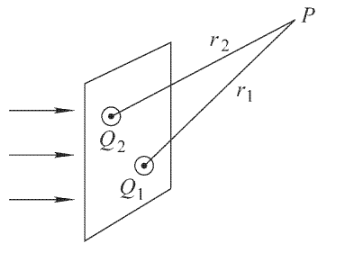
\includegraphics[width=0.27\textwidth]{figures/31_1.png}
    \caption{Расчёт пространственной и временной когерентности.}
    \label{fig:31}
\end{figure}


\textbf{Оборванная синусоида}. Пусть есть $\sin$ вплоть до некоторого $\tau$ по которому и будем усреднять
\begin{equation*}
    E(t) = \left\{\begin{aligned}
        &\sin \omega_0 t, &t \in[0, \tau], \\
        &0,     &t \notin [0, \tau],
    \end{aligned}\right.
    \hspace{0.5cm} \Rightarrow \hspace{0.5cm}
    \gamma(\theta) = \left\{\begin{aligned}
        &1-\theta/\tau, &\theta < \tau, \\
        &0, &\theta > \tau.
    \end{aligned}\right.
\end{equation*}
что может быть получено из выражения
\begin{equation*}
    \left\langle E(t) E^* (t-\theta)\right\rangle = \frac{1}{\tau} \int_0^\tau e^{i \omega_0 \theta} \d t = \frac{\tau-\theta}{\tau} e^{i \omega_0 \theta} = F(\theta) = f(\theta).
\end{equation*}
\red{Вот здесь написать подробнее.}

\textbf{Связь автокорреляционной функции и спектральной плотности}. Да, они связаны: $F(\theta)$ и $I_\omega(\omega)$. Для установления связи запишем по определению
\begin{equation*}
    F(\theta) = \left\langle E(t) E^* (t-\theta)\right\rangle = \frac{1}{\tau} \int_{-\tau/2}^{\tau/2} E(t) E^* (t-\theta) \d t,
\end{equation*}
подтсавляя $E^*(t-\theta) = \int_0^\infty a^* (\omega) e^{-i \omega (t-\theta)} \d \omega$, а также вспоминая выражения для $a(\omega)$, и меняя порядок интегрирования приходим к
\begin{equation*}
    a(\omega) = \frac{1}{2\pi} \int_{-\tau/2}^{\tau/2} E(t) e^{-i \omega t} \d t,
    \hspace{0.5cm} \Rightarrow \hspace{0.5cm}
    F(\theta) = \frac{2\pi}{\tau} \int_{0}^{+\infty}  a^*(\omega) a(\omega) e^{i \omega \theta} \d \omega = 
    \int_{0}^{\infty} I_\omega (\omega) e^{i \omega \theta} \d \omega,
\end{equation*}
где учтено, что $I_\omega (\omega) = \frac{2\pi}{\tau} a^*(\omega) a(\omega)$. Это формула -- фурье-разложение $F(\theta)$, поэтому верно и обратное
\begin{equation*}
    F(\theta) = \int_{0}^{\infty} I_\omega (\omega) e^{i \omega \theta} \d \omega,
    \hspace{0.5cm} \Rightarrow \hspace{0.5cm}
    I_\omega (\omega) = \frac{1}{2\pi} \int_{-\infty}^{+\infty} F(\theta) e^{-i \omega \theta} \d \theta.
\end{equation*}
Вообще можно показать, что $F(-\theta) = F^*(\theta)$, тогда последняя формула перепишется в виде:

\begin{to_thr}[теорема Винера-Хинчина]
    Связь между спектральной плотностью мощности сигнала и его автокорреляционной функцией может быть записана в виде:
    \begin{equation*}
    I_\omega (\omega) = \frac{1}{2\pi}\left[
        \int_{0}^{\infty} F(\theta) e^{- i \omega \theta} \d \theta + \text{c.c.}
    \right],
    \end{equation*}
    что позволяет измерять $I_\omega$ для волн.
\end{to_thr}

% Так можно мерять $I_\omega$!